The UML diagram does not show what to do first and next or how to design the system but it helps to visualize the structure and the communication between objects.
It is on the problem-side domain, which means it is used to get a general view of the system to be developed through the understanding of objects concepts and properties.

On the present scenario, there are four agents identifiable across the \glsfull{mtemsm} and one agent under the blockchain system.
The former has the three access type to the available \gls{mtemsm} information -- the general person, the general user and the member -- plus the group consensus.
The later has only the blockchain consensus responsible for what will be appended or not on the ledger.

The associations guide either singular and plural relationships between agents, and how entities relate to each other.
However, only the most relevant relationships between agents and entities are considered, for instance, some attributes of power plants can be updated through the same way as the request to change a member register, so the display of this relation was avoided.
Similarly happens to the request to delete a member or a power plant register from the group storage space.
The association notation towards the entity \verb|New Values| highlights these relationship constraints.

Moreover, the relationships between general person, general user and member are based on the consensus considered to update their access attribute to the ledger information.
This association is prefered in spite of the definition of each other as a specialization.
This procedure is important indeed to highlight that any general user is not identifiable by its real ID attribute at the blockchain ledger. But a member can be so inside the \gls{mtemsm} context.
The opposite happens with the \verb|Referendum Process| that is a generalisation of any request to change a value in the \gls{mtemsm} storage space.
It will always create a unique identification for every request and wait for the group consensus to take action.

Another association to be considered is the external interface.
Any trade process upon an agreement must be held off-chain independently of how it will be.
If the platform is a power auction or e-marketplace does not really matter but only the check-out step to formalize the trade must happen on-chain.
This methodology can be extended to the waiting period needed to accomplish with a given purpose.
The blockchain does not have a time counting function to determine when another operation should be performed.
However, it makes instantaneous analysis to allow or not a given operation to happen.

Lastly, the black diamonds indicate an object is responsible for the existence and storage of the associated object.
This composite aggregation means that a part belongs to at most one object, for instance, there is only one group consensus by each referendum process or even the construction of a new power plant depends solely on its crowdfunding.

\begin{figure}{\textwidth}
    \centering
    \frame{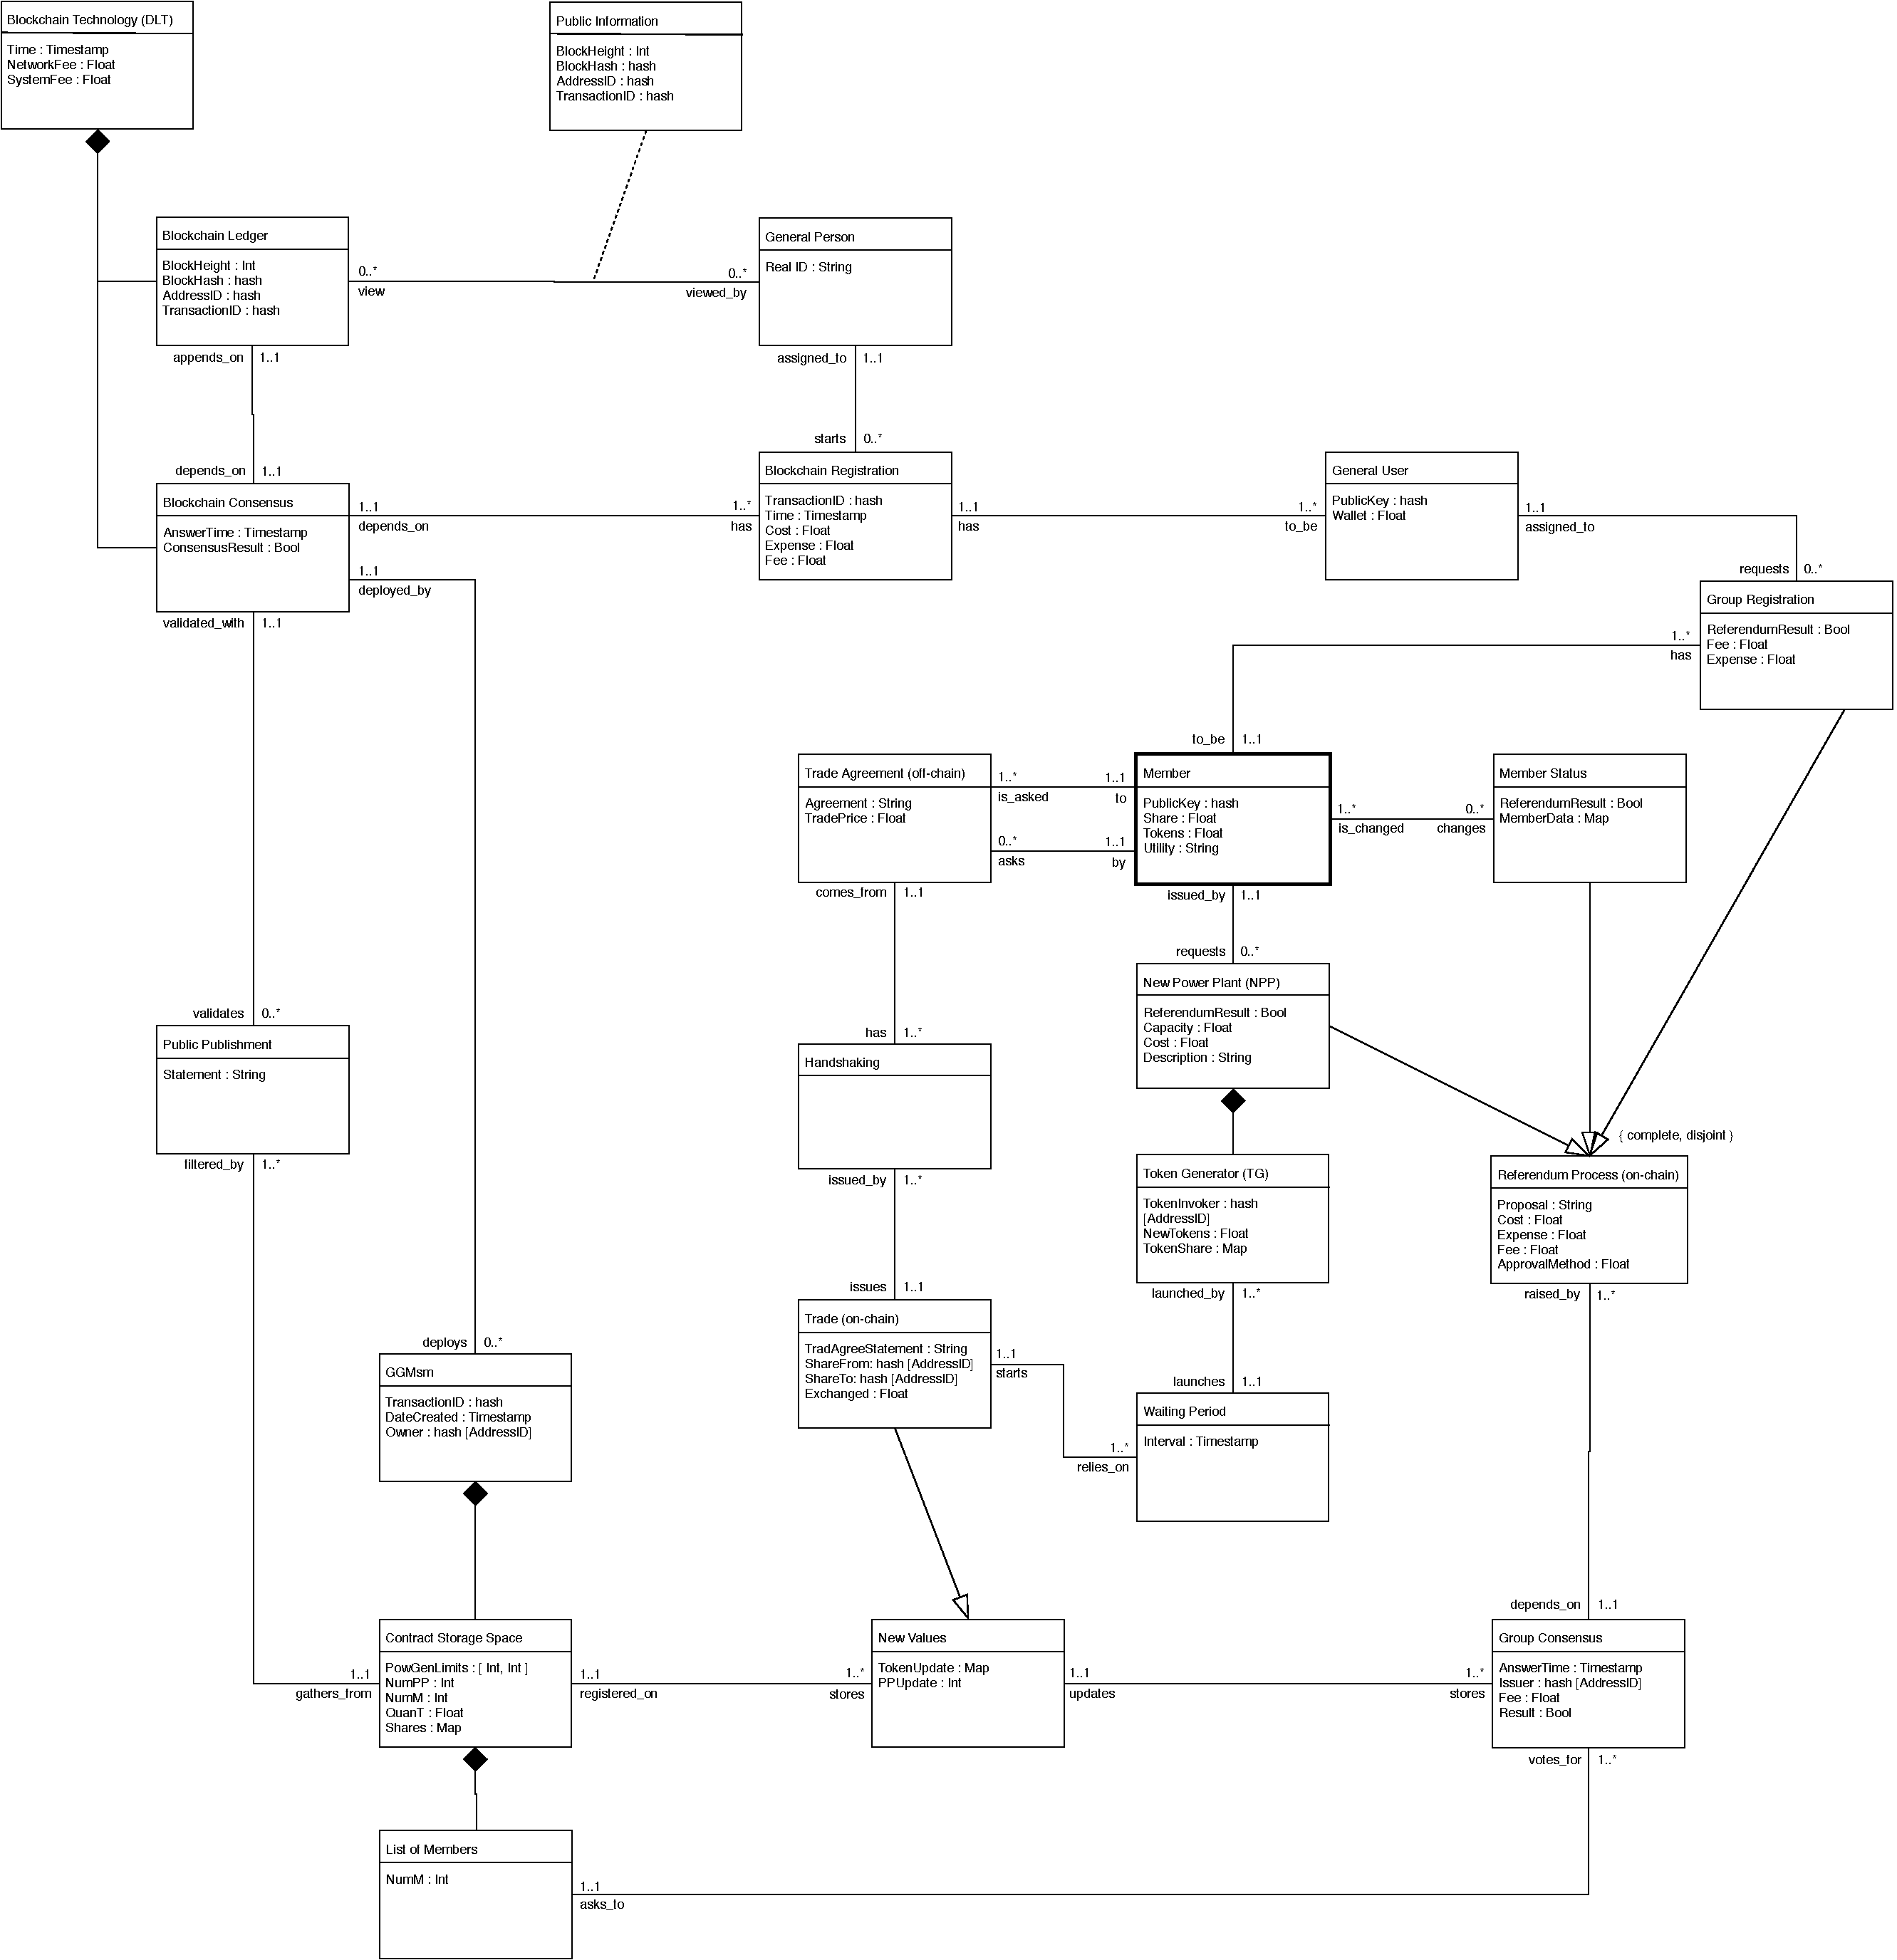
\includegraphics[width=\textwidth]{uml}}
    \caption{\Gls{uml} diagram of the distributed application proposed.}
    \label{fig:uml}
\end{figure}

% https://trello.com/c/0UYt6Nvp/144-uml-class-diagrams-for-software-engineering

% https://www.draw.io/?state=%7B%22ids%22:%5B%221y3X9DgbtlhgImNH5nZjBE9l8SDTSGMoy%22%5D,%22action%22:%22open%22,%22userId%22:%22115555534608635891757%22%7D#G1y3X9DgbtlhgImNH5nZjBE9l8SDTSGMoy